\documentclass[conference,10pt]{IEEEtran}
\usepackage{fancyhdr}
\usepackage{amssymb}
\usepackage{amsmath}
\usepackage{amsfonts}
\usepackage[T1]{fontenc} % get tt fonts to work right
\usepackage{graphicx}
\usepackage{fixltx2e}
\usepackage{multirow}
\usepackage{color}
\usepackage{caption}
\DeclareCaptionType{copyrightbox} % workaround for bug in caption
\usepackage{subcaption}
\usepackage{xspace}
\usepackage{url}

\begin{document}

\special{papersize=8.5in,11in}
\setlength{\pdfpageheight}{\paperheight}
\setlength{\pdfpagewidth}{\paperwidth}


\title{Mapping HALO Exchange onto Toruses and Stuff}

\author{\IEEEauthorblockN{
Yadu N. Babuji\IEEEauthorrefmark{1}\IEEEauthorrefmark{2}\IEEEauthorrefmark{3},
Timothy G. Armstrong\IEEEauthorrefmark{1}}
  \IEEEauthorblockA{
  \IEEEauthorrefmark{1}Dept. of Computer Science,
    University of Chicago,
    Chicago, IL, USA}
  \IEEEauthorblockA{\IEEEauthorrefmark{2}Mathematics and Computer Science Division,
    Argonne National Laboratory,
    Argonne, IL, USA}
  \IEEEauthorblockA{\IEEEauthorrefmark{3}Computation Institute,
    University of Chicago and Argonne National Laboratory,
    Chicago, IL, USA}
}

\maketitle


\begin{abstract}
% Motivation
Many High Performance Computing (HPC) applications involve application domain decompositions that involve nearest neighbour communication.
Halo exchange is a common nearest neighbor communication pattern used for solving PDE's and thus applying to a wide range of HPC applications.
% Problem statement % Approach
Empirical results show that different task placement strategies in Halo exchange codes can have as much as 7.5x performance difference.
We develop an analytical model to understand the impact of task placements withing a network topology on performance and guide selection of
optimal mappings.
% Results
Analytic model comes with x percentage of empirical results with a max error of E.
Identified optimal and pessimal mappings.
% Conclusions


[TODO]
\end{abstract}

\section{Introduction}

% Intro
Halo exchange is a common communication pattern in parallel codes, where
each process is assigned an application subdomain and must periodically
communicate with other processors that have neighboring subdomains to
update information about the state of the boundary between subdomains.
A common special case is when a multi-dimensional cartesian space is
decomposed into subdomains of equal size.  For example, in the three-dimensional
case, a 8x8x8 cube might be decomposed into 256 2x1x1 cubes for execution on 256 processors.

% Objective
This paper explores the problem of mapping such multi-dimensional cartesian
halo exchange communications onto parallel computers with hypercube or
torus networks. A typical computation job on a leadership class machine would
utilize several hundreds to thousands of cores, as a result there are a large number of
possible mappings to the physical hardware that could be chosen. We seek to understand
what aspects of the mappings have an impact on performance and how to quantify them so
that the impact these mappings have on performance can modelled. Mapping strategies
are a very cheap optimisation which requires no code changes to the application
and as our empirical studies show, these mapping stategies have significantly
different network performance characteristics. There are no studies to the best
of our knowledge that attempts to model the impact of mapping performance on
HPC systems.

% What does this paper contribute:
TODO\\
1. An analytical model that describes the perfomance on Halo exchange with different mappings\\
2. A nearly worst and optimal mapping.\\

The rest of the paper is organised as follows :
% Guidance
The rest of the paper is organised as follows: Section 2, provides background information on
the HPC system topologies and BlueGene/Q in particular. Section 3, describes mapping strategies.
Section 4, develops the analytical model and Section 5, details the experiment design for empirical
validation of the model.

% Summary conclusions

\section{High-Performance Computer Networks}

The state of the art in High Performance Computing(HPC) infrastructure, demands high-performance networks
to support the movement of data between the nodes as well as to-and-from disk-arrays. HPC systems are
increasingly architected with high radix interconnects such as hypercubes and N-dimensional tori.
Parallel applications have a wide range of task placements options to exploit the network topology of
these HPC systems. These networks have evolved to several different network topologies in order to support
different requirements, and data movement patterns. For HPC applications which involve fine-grained communication,
high-radix networks provide low latency, smaller diameter, and large bandwidth as multiple links along the multiple
dimensions supprted.

% Routing protocols on the BG/Q
% Direct routing
% Adaptive routing
\subsection{Blue Gene/Q 5D torus network}

The BlueGene/Q is a 3rd generation massively parallel supercomputer from IBM. The BlueGene/Q implements a 5 dimensional torus with upto 16K nodes.
To support the 5 dimensional torus each compute node has 10 bi-directional duplex links. There is a separate 11th link for IO. Each of the 10 links
operate at a bandwidth of 2GB/s \cite{BGQ_RedBook_2013}. After accounting for 10\% overhead in message headers 1.8GB/s is available for raw data per link in one-direction.
The 5D torus network provides high nearest neighbor bandwidth as well bisection bandwidth while decreasing the maximum number of hops to reach
the furthest nodes. The dimensions on the network are labelled as A,B,C,D,E and the cores on the node using T. The E dimension is limited to a length
of 2, while A,B,C,D dimensions can be multiples of 4 to remain torus. The intranode per hop latency is approximately 40ns BGQ \cite{BGQ_Interconnect_2012}
while the worst point-to-point network latency is expected to be under 3$\mu$s. 

% The BGQ routing protocols
The BlueGene/Q implements two routing protocols for point-to-point communication.
Deterministic routing is designed for small messages, where packets sent between two nodes take the same direct path.
This routing method is prone to creating hotspots when traffic between several nodes cross on some node.
Adaptive routing determines the route for packets at the runtime taking current network loads into consideration.
This routing mechanism balances the network load for a penalty in latency.


\subsection{Message Passing Interface(MPI)}
The Message Passing Interface (MPI) is a standard for message-passing in HPC applications.
We use MPI to implement the messaging and synchronization aspects of the HALO exchange code,
and hence the performance observed from running the application would be influenced by the behavior of MPI due to it's various protocols on the BlueGene/Q.
There are four protocols supported by the MPI implementation used BlueGene/Q.
The protocol utilized by MPI is determined by the size of the message that is being sent.
The data sizes at which the switch to different protocol occurs is configurable, but for our experiments we use the defaults on BlueGene/Q.

% Add note on : Intranode latency implemented as in-memory copy
% Large message copies as RDMA copy.
MPICH2 Nemesis.

\begin{table}
  \caption{MPI Protocol default thresholds}
    \begin{tabular}{ | l | l | l | p{2cm} |}
    \hline
    Protocol   & Min Data Limit & Max Data Limit & Routing\\ \hline
    Immediate  &             0B &           112B & Direct\\ \hline
    Short      &           113B &           496B & Direct\\ \hline
    Eager      &           497B &          4096B & Direct\\ \hline
    Rendezvous &          4096B &      unlimited & Adaptive\\ \hline
    \hline
    \end{tabular}
\end{table}

\section{Mapping Strategies}

Different classes of HPC systems provide different mechanisms and varying levels of control on task placement.
The MPI framework gives finegrained control of placement of tasks via a mapping file when such functionality
is supported by the hardware. On BlueGene/Q systems from IBM, the mapping files allow you to determine where
each MPI rank is placed within a machine partition. On Cray XE6 machines, which do not have the notion of
isolated machine partitions, the mapping functionalities only give the flexibility of choosing the node on
which a set of ranks will execute on, but not the physical proximity of the nodes with relation to each other.
The Cray XE6 does not guarantee isolation of the network from the traffic generated by other users and it
also cannot guarantee that the location of nodes with relation to the rest of the nodes would remain constant
across multiple runs. As a result BlueGene/Q systems can offer far greater control on task placements, and
better guarantees on reproducible results.

With the focus on BlueGene/Q systems here's a broad outline of different mapping strategies we have examined:

\subsection{Regular/Default Mapping}
The default mapping involves ranks being assigned in increasing order along the dimensions T, E, D, C, B, A.
Assuming that we assign 16 ranks with one rank per core, the first 16 ranks from the application domain will
be on the node with address (0 0 0 0 0) and so on. Since the ranks in the application domain are assigned in
some increasing order, nodes along a particular dimension will be grouped on each node. This mapping works
very well when the dimensionality of the application domain and that of the partition match. For eg, if the
application domain were 4x4x4x4x2 and we were running one rank per node, there is a one to one mapping to the
network where this mapping would retain nearness between all neighbors. However when the length of dimensions
in the application domain and network or the dimensionality do not match, this mapping scheme might not be
optimal.

\subsection{Linear Mapping}
Linear mapping refers to placing ranks along nodes in the increasing order of dimensions A, B, C, D, E, T.
As a result the neighboring ranks in the application domain along a dimension are places on nodes atleast
one hop away.

\subsection{Skewed Mapping}

\subsection{Random Mapping}
\subsection{Mappings from Simulated Annealing}
\subsection{Mappings from }



\section{Models for Network Communication}

On an HPC system such as BlueGene/Q or Cray XE6, each node has multiple duplex links to it's neighbors.
If the application on every node attempts to exchange messages with every neighbor, we can assume that
every link on the network will see similar traffic. Thus we, consider a single link and it's bandwidth
to determine t\textsubscript{b} the time required to send a Byte along the link. Assume that there are N\textsubscript{procs} number
of identical processes all of which will attempt to utilize the same links. To capture the differences
between different mappings we use a simple program to calculare the average distance between neighbors,
N\textsubscript{steps}. The current MPI implementation on leadership class systems like Mira (Bluegene/Q) utilizes
shared memory for intranode communication. When a neighbor is present within the same node, the link
is weighted as zero, and every network link or hop is weighted as one. Since it is possible to place
neighboring tasks from the application domain on the same node there are mappings possible which
minimize N\textsubscript{steps} below one. There are constant costs involved in startup, acquiring a buffer etc,
and t\textsubscript{c} is an experimentally calibrated constant that is a catch-all for the various constant costs
of network communication using MPI. N is the message size in bytes that are exchanged between neighbors.

A simple analytical model determines the time to completion, T of a complete halo exchange operation,
from the variables defined above as follows:

\begin{equation}
  T = t_c + (N_{steps} * N_{procs} * N * t_b)
\end{equation}

Since we have a complex set of operations on several hundreds of nodes, there is a cost for synchonisation.
We use MPI barriers to synchronise all tasks before and after measurements

\section{Experimental Design}

\label{sect:3D Halo plot}
\begin{figure}
  \center
  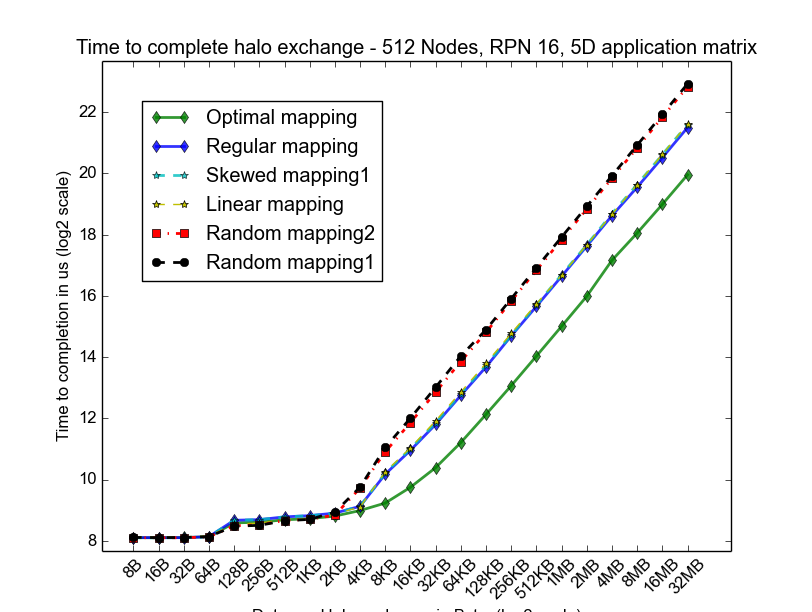
\includegraphics[width=0.5\textwidth]{5D_512_most_mappings_2.png}
  \caption{5D halo exchange on 512 nodes with 16 RPN}
    \label{fig:3D halo exchange on 512 nodes with 16 RPN}
\end{figure}


\section{Results}

\section{Conclusion}


\bibliographystyle{abbrv}
\bibliography{halo}

\end{document}
